\documentclass[tikz,border=10pt]{standalone}
\usepackage{mathrsfs}
\usepackage{physics}
\usetikzlibrary{decorations.pathmorphing}
    % this is for graphics. e.g. rectangle on title page
\usetikzlibrary{3d}
\usetikzlibrary{backgrounds}
\usetikzlibrary{arrows,shapes,positioning,shadows,trees,mindmap}
\usetikzlibrary{tikzmark}
\usetikzlibrary{calc,math}

\usepackage{tikz-3dplot}
\usepackage{pgfplots}
\pgfplotsset{compat = newest}
%\usepgfplotslibrary{colormaps}
\usepgflibrary{shapes.geometric}

\usepackage[edges]{forest}
\usetikzlibrary{arrows.meta}
\colorlet{linecol}{black!75}
\usepackage{xkcdcolors} % xkcd colors

\usetikzlibrary{patterns}
\tikzset{>={Stealth[inset=0pt,angle=20:10pt]}}


\tikzset{zigzag/.style={decorate,decoration=zigzag}}


\begin{document}
\tikzset{every picture/.style={line width=0.75pt}} %set default line width to 0.75pt        

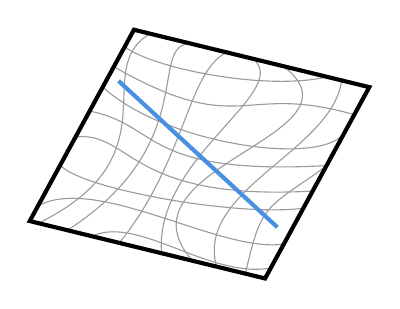
\begin{tikzpicture}[x=0.75pt,y=0.75pt,yscale=-0.45,xscale=0.45]
%uncomment if require: \path (0,300); %set diagram left start at 0, and has height of 300

%Curve Lines [id:da47768964797134705] 
\draw [color={rgb, 255:red, 155; green, 155; blue, 155 }  ,draw opacity=1 ]   (46.5,219) .. controls (189,127.2) and (132.2,21.6) .. (177.4,19.2) ;
%Curve Lines [id:da2372020035028457] 
\draw [color={rgb, 255:red, 155; green, 155; blue, 155 }  ,draw opacity=1 ]   (102.33,232) .. controls (172.33,145.33) and (175,49.33) .. (216.07,29.2) ;
%Curve Lines [id:da15350016006086475] 
\draw [color={rgb, 255:red, 155; green, 155; blue, 155 }  ,draw opacity=1 ]   (147,243.33) .. controls (139,143.33) and (283.67,72.67) .. (246.73,37.2) ;
%Curve Lines [id:da46035703072596923] 
\draw [color={rgb, 255:red, 155; green, 155; blue, 155 }  ,draw opacity=1 ]   (15.17,211.67) .. controls (162.33,139.33) and (69,46.67) .. (135,8.67) ;
%Curve Lines [id:da793584433912975] 
\draw [color={rgb, 255:red, 155; green, 155; blue, 155 }  ,draw opacity=1 ]   (179.67,251.33) .. controls (93,152) and (370.33,118) .. (279.4,45.2) ;
%Curve Lines [id:da009602049360326825] 
\draw [color={rgb, 255:red, 155; green, 155; blue, 155 }  ,draw opacity=1 ]   (205.75,257.25) .. controls (183.75,175.92) and (328.33,134.67) .. (339.67,60) ;
%Curve Lines [id:da023428392508223927] 
\draw [color={rgb, 255:red, 155; green, 155; blue, 155 }  ,draw opacity=1 ]   (237,264.67) .. controls (254.33,189.33) and (257.67,197.33) .. (324.33,150) ;
%Curve Lines [id:da23198885835653482] 
\draw [color={rgb, 255:red, 155; green, 155; blue, 155 }  ,draw opacity=1 ]   (14.33,193.33) .. controls (77,158.67) and (210.33,244) .. (277,234) ;
%Curve Lines [id:da9320547769035521] 
\draw [color={rgb, 255:red, 155; green, 155; blue, 155 }  ,draw opacity=1 ]   (39.67,150.67) .. controls (67,176.67) and (233.67,205.33) .. (300.33,195.33) ;
%Curve Lines [id:da6832216440778782] 
\draw [color={rgb, 255:red, 155; green, 155; blue, 155 }  ,draw opacity=1 ]   (71.67,226) .. controls (120.33,202) and (195.67,270) .. (262.33,260) ;
%Curve Lines [id:da25287123249566745] 
\draw [color={rgb, 255:red, 155; green, 155; blue, 155 }  ,draw opacity=1 ]   (54.33,119.33) .. controls (115,112.67) and (110.33,188) .. (307,177.33) ;
%Curve Lines [id:da4546460716170495] 
\draw [color={rgb, 255:red, 155; green, 155; blue, 155 }  ,draw opacity=1 ]   (71.67,92) .. controls (145.67,107.33) and (127.67,160.67) .. (324.33,150) ;
%Curve Lines [id:da37921397456508843] 
\draw [color={rgb, 255:red, 155; green, 155; blue, 155 }  ,draw opacity=1 ]   (85,66.67) .. controls (148.33,124.67) and (309,150.67) .. (341,117.33) ;
%Curve Lines [id:da14363350141795972] 
\draw [color={rgb, 255:red, 155; green, 155; blue, 155 }  ,draw opacity=1 ]   (97,44.67) .. controls (233,122) and (231.67,60.67) .. (353,95.33) ;
%Curve Lines [id:da8613527515020676] 
\draw [color={rgb, 255:red, 155; green, 155; blue, 155 }  ,draw opacity=1 ]   (107,22.67) .. controls (143,48) and (263.67,70) .. (325.67,54.67) ;
%Straight Lines [id:da5177592290443334] 
\draw [color={rgb, 255:red, 74; green, 144; blue, 226 }  ,draw opacity=1 ][line width=1.5]    (101,59.33) -- (271,216) ;
%Flowchart: Data [id:dp8794166896502564] 
\draw  [line width=1.5]  (117.47,4.53) -- (369.43,65.99) -- (257.86,270.82) -- (5.9,209.35) -- cycle ;
\end{tikzpicture}
\end{document}